\begin{center}
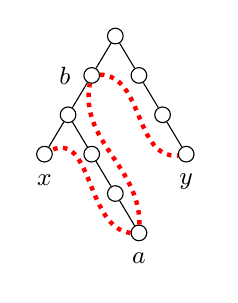
\begin{tikzpicture}[scale=.5,level distance=10mm, state/.style={circle, draw, minimum size=1mm}]]
  \tikzstyle{every node}=[font=\small, draw=black,circle,inner sep=2pt, minimum size=1mm]
  \tikzstyle{level 1}=[sibling distance=12mm, set style={{every node}+=[draw=black]}]
  \tikzstyle{level 2}=[sibling distance=12mm, set style={{every node}+=[draw=black]}]
  \tikzstyle{level 3}=[sibling distance=12mm,  set style={{every node}+=[draw=black]}]
  \tikzstyle{level 4}=[sibling distance=12mm,  set style={{every node}+=[draw=black]}]
  \tikzstyle{level 5}=[sibling distance=12mm,  set style={{every node}+=[draw=black]}]
  \tikzstyle{level 6}=[sibling distance=12mm,  set style={{every node}+=[draw=black]}]

    \node (u) {}
     child {
        node[label=left:{$b$}] (b) {}
              child {node (B) {}
                child {node (x)[label=below:{$x$}] {}
        %         child {node (v) {}}
        % child {node (E) {}}
       }
       child {node (F) {}
        child[fill=none] {edge from parent[draw=none]}
        child {node (G) {}
            child[fill=none] {edge from parent[draw=none]}
            child {node[label=below:{$a$}] (a) {}}
            }
      }}
      child[fill=none] {edge from parent[draw=none]
       child[fill=none] {edge from parent[draw=none]
        child[fill=none] {edge from parent[draw=none]}
        child[fill=none] {edge from parent[draw=none]}
        }
       child[fill=none] {edge from parent[draw=none]
        child[fill=none] {edge from parent[draw=none]}
        child[fill=none] {edge from parent[draw=none]}
       }
      }
      }
      child {node{}
       child[fill=none] {edge from parent[draw=none]
        child[fill=none] {edge from parent[draw=none]
         child[fill=none] {edge from parent[draw=none]}
         child[fill=none] {edge from parent[draw=none]}
         }
       child[fill=none] {edge from parent[draw=none]
        child[fill=none] {edge from parent[draw=none]}
        child[fill=none] {edge from parent[draw=none]}
       }
      }
       child[fill=none] {node {}
        child[fill=none] {edge from parent[draw=none]
         child[fill=none] {edge from parent[draw=none]}
         child[fill=none] {edge from parent[draw=none]}
        }
       child[fill=none] {node[label=below:{$y$}] (y) {}
        child[fill=none] {edge from parent[draw=none]}
        child[fill=none] {edge from parent[draw=none]}
        }
       }
       };

    
    \draw[-,dotted,ultra thick,relative,red] (a) to[out=40,in=250] (x);
    
    \draw[-,dotted,ultra thick,relative,red] (a) to[out=-20,in=150] (b);

    \draw[-,dotted,ultra thick,relative,red] (b) to[out=45,in=230] (y);
       
\end{tikzpicture}
\end{center}